\documentclass[10pt,letterpaper,addpoints]{exam}
\usepackage[utf8]{inputenc}
\usepackage[spanish,es-noshorthands]{babel}
\usepackage{hyperref}
\usepackage{amsmath}
\usepackage{amsfonts}
\usepackage{amssymb}
\usepackage{graphicx}
\usepackage{tikz}
\usepackage{multicol}
\usepackage[width=7in,height=9.5in]{geometry}
%\printanswers
\begin{document}
\title{\begin{minipage}{.2\textwidth}
        
\includegraphics[height=1.75cm]{Images/logo-colegio.png}
       \end{minipage}
\begin{minipage}{.55\textwidth}
 \begin{center}
Prueba bimestral \\Álgebra $8^{\circ}$
\end{center}
\end{minipage}
\begin{minipage}{.2\textwidth}

\includegraphics[height=1.75cm]{Images/logo-sed.png} 
\end{minipage}
}
\author{Germ\'{a}n Avendaño Ram\'{i}rez\\Lic. Matemáticas U.D., M.Sc. U.N.}
\date{}
\maketitle
\begin{center}
\fbox{\fbox{\parbox{5.5in}{\centering
Instrucciones}}}
\end{center}
\vspace{0.1in}
\makebox[\textwidth]{Nombres: \hrulefill, curso:\underline{\hspace{48pt}}, fecha:\underline{\hspace{3cm}}}
\begin{questions}
\begin{minipage}{.65\textwidth}
\question
Una máquina corta moldes de cartón que se doblan y se pegan para construir cajas, con las medidas que se muestran en el siguiente dibujo.\\

¿Cuál de las siguientes cajas se arma con el molde del dibujo?
\end{minipage}\hfill
\begin{minipage}{.35\textwidth}
\begin{tikzpicture}
\draw (0,0) rectangle (4,1);
\draw (1,-2) rectangle (3,2);
\draw (1,-1)--(3,-1);
\draw[|-] (-.2,1)--node[below]{10cm}(-.2,.6);
\draw[|-](-.2,0)--(-.2,.4);
\draw[|-](0,-.2)--node[right]{10cm}(.1,-.2);
\draw[-|](.9,-.2)--(1,-.2);
\draw[|-](1,-2.2)--(1.5,-2.2)node[right]{20cm};
\draw[-|](2.5,-2.2)--(3,-2.2);
\draw[|-](3.2,-.1)--(3.2,-.4)node{10cm};
\draw[-|](3.2,-.6)--(3.2,-1);
\end{tikzpicture}
\end{minipage}
\begin{center}
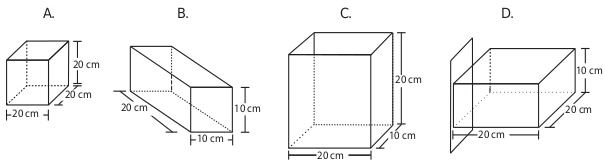
\includegraphics[scale=.75]{Images/cajas.png} 
\end{center}
\begin{minipage}{.35\textwidth}
\question
En un juego Juan lanzó tres dardos a un tablero como el siguiente:\\

El puntaje del juego se obtiene sumando los puntos asignados a la posición donde cae cada dardo.

Los tres dardos que lanzó Juan quedaron ubicados en los recuadros E5, F6 y D7.\\

¿Qué puntaje obtuvo Juan?
\end{minipage}\hfill
\begin{minipage}{.65\textwidth}
\begin{center}
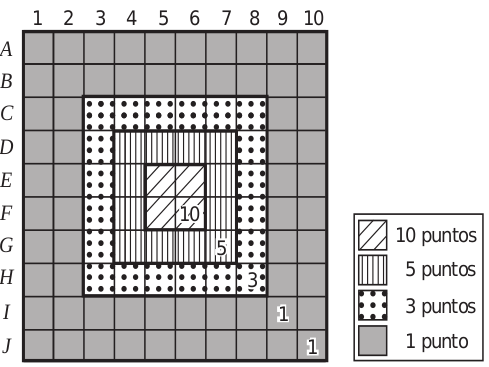
\includegraphics[scale=.55]{Images/juego_dados.png} 
\end{center}
\end{minipage}

\begin{oneparchoices}
\choice 15 puntos.
\choice 18 puntos.
\choice 20 puntos.
\CorrectChoice 25 puntos.
\end{oneparchoices}

\begin{minipage}{.5\textwidth}
\question 
La siguiente tabla muestra los nombres de los atletas de un equipo y sus respectivos pesos.

El equipo realiza algunos ejercicios en parejas. La diferencia de pesos entre los atletas que conforman una pareja no debe sobrepasar los 3 kilogramos.

¿Cuáles de los siguientes atletas del equipo \textbf{no} pueden realizar los ejercicios en pareja?
\end{minipage}\hfill
\begin{minipage}{.5\textwidth}
\begin{tabular}{|c|c|}
\hline 
\textbf{Nombre del atleta} & \textbf{Peso en kilogramos} \\ 
\hline 
Oscar & 60 \\ 
\hline 
Andrés & 62.5 \\ 
\hline 
Víctor & 58.6 \\ 
\hline 
Fernando & 61.3 \\ 
\hline 
César & 65.2 \\ 
\hline 
Héctor & 59.4 \\ 
\hline 
\end{tabular} 
\end{minipage}

\begin{oneparchoices}
\choice Oscar y Víctor.
\choice Fernando y Héctor.
\CorrectChoice César y Víctor.
\choice Andrés y Fernando.
\end{oneparchoices}
%\answerline
\end{questions}
%cuadro de puntajes
%\begin{center}
%\gradetable[h][pages]
%\end{center}
\end{document}